\documentclass[a4paper]{article}
\usepackage{listings}
\usepackage{graphicx}
\begin{document}

\title{COMP343 Assignment 2:\\
Security analysis of Android APK file format \\
and associated technologies within the\\
Android Operating System}
\date{Monday Jun 3, 2013}
\author{Adam Carmichael \\
adam.carmichael@mq.edu.au \\
Department of Engineering \\
Macquarie University}
\maketitle

\tableofcontents

\section{Summary}
Android APK File Format - a zip file format used to package applications onto an
Android device such as a tablet, phone, or smart television / set top box.
\\
\\
\noindent APK files must have several specific directories and files, some of
which are of interest as they maintain the security through cryptographic certificates and
hash functions, others will only be mentioned in summary as they are of minimal
interest in the context of this assignment.
\\
\\
\noindent This document does not cover exploits where by the default install permitted
network operators to send SMS codes to reset the phone to a default state, or to
install arbitrary software and attempts to focus on the APK File Format and the
permissions and access control structure surrounding it.

\section{Detailed Description}
The APK file format contains the following tree layout:
\begin{lstlisting}
.
+-- AndroidManifest.xml
+-- assets
+-- classes.dex
+-- META-INF
|   +-- CERT.RSA
|   +-- CERT.SF
|   +-- MANIFEST.MF
+-- res
|   +-- anim
|   +-- drawable
|   +-- layout
|   +-- xml
+-- resources.arsc
\end{lstlisting}

\begin{itemize}
  \item \texttt{AndroidManifest.xml} is a compiled XML file and is not human
  readable, but it may be converted to XML using a tool such as
\texttt{apktool}\footnote{https://code.google.com/p/android-apktool/}.
The \texttt{AndroidManifest.xml} file contains information such as the application
name, and access rights (called permissions) that the application would like to
use. These permissions are presented to the user when the user goes to install
the application, and are also shown in the Google Play Store (and other markets)
when the user can browse the application. A user can opt to not install an
application if it uses a permission the user is not willing to grant (such as
send an SMS).

  \item \texttt{assets} are things such as sounds that the application may need
to use.

  \item \texttt{classes.dex} Android operates a virtual machine called Dalvik
  which shares many similarities with Java. A \texttt{.dex} file is a Dalvik executable
can be thought of as similar to a \texttt{.class} file in Java.

  \item \texttt{META-INF} is a directory which contains the following three
  files of interest:
\begin{itemize}
  \item \texttt{MANIFEST.MF} a listing of all files present in the APK and a
  digest of their content (default hash algorithm is SHA-1 represented as a
  base64 value).
  \item \texttt{CERT.RSA} application certificate. Standard \texttt{openssl}
  commands from the Linux command line can be used to read and verify these
  certificates.
  \item \texttt{CERT.SF} a \texttt{SHA-1} hash of each entry in the
  \texttt{MANIFEST.MF} file, which is then signed using the application
  certificate, \texttt{CERT.RSA}. 
  \end{itemize}
  
  Typically, in signing an \texttt{APK}, the compiled application is SHA-1
  hashed (\texttt{MANIFEST.MF}), and then the hash entries are hashed as second
  time, signed using \texttt{CERT.RSA} to produce the signature file
  \texttt{CERT.SF}.
  
\end{itemize}

\noindent When an application is to be installed, it is done using the Package
Manager within the operating system, which places calls to check \texttt{CERT.SF}. It
also includes the prompt to the user showing the permissions required from
\texttt{AndroidManifest.xml}, and this presents the weakest point of the
security system - the end user.

\section{Assets at Risk}
Three assets that may be placed at risk are
\begin{itemize}
  \item Phones
  \item Tablets
  \item Digital TVs / set top boxes
\end{itemize}

\noindent If one uses their phone or tablet for banking, and an attacker
installs malicious software onto the victim's device, it is possible that banking data
could be exposed. By the same token, confidential email data may be leaked, or,
more simply, a phone could be turned into a zombie bot for sending SMS
spam messages.

\noindent Information leakage is possible despite software running in sandboxed
processes. One possible example of defeating the sandbox is to install a
replacement keyboard - thereby reading all keystrokes.

\section{Threat Surface}
Three possible attack vectors in which an adversary may comprimise a device:
\begin{itemize}
  \item Social engineering - asking a user to install a piece of malicious
  software under some false pretense.
  \item Physically obtaining the handset in an unlocked state and installing a
  piece of malicious software, perhaps in a socially engineered attempt to 'fix
  a problem'.
  \item Remote attack on running daemons - some handsets run the Dropbear SSH
  daemon; if this daemon runs as root and were to be comprimised (say buffer
  overflow), packages can be installed into the system partition and run at the
  next reboot.
\end{itemize}

\section{Vulnerabilities}
\noindent In two of these three possible attack vectors, the attacker is
required to either have the device, or to trick the end user into installing software onto
the device.
\\
\noindent Users must exercise discretion when installing software, and be
cautious who they hand their unlocked devices to.
\\
\noindent The third vulnerability is the most interesting, as it requires
exploiting bugs in software that may not be running on the device. Attacks can be mitigated by
turning off daemons that are not necessary (most users are not running Dropbear
SSH by default).
\\
\noindent Versions of Android prior to 4.0 can be plugged into a desktop
computer and enter a debug mode whereby packages can be installed over a USB cable (this is
also available over IP) using \texttt{ADB}\footnote{Android Debug Bridge}
without a prompt from the user. This is typically turned off by default. More
recently, on screen prompts to show the application permissions became the norm,
however most recently, a handshake procedure between the handset and the
computer similar to the SSH host key authentication process takes place. If a PC
is not trusted, \texttt{ADB} refuses the connection and software cannot be
installed.

\section{Controls}
The \texttt{AndroidManifest.xml} file presents a list of requested permissions
that an APK requires to run, and at install time the list of permissions is
shown to the user so they can determine if the end user should install the
software or not. \textbf{Figure \ref{fig:install-time}} shows the permissions
listed in the \texttt{AndroidManifest.xml} for an application called \textbf{Remote for VLC}.
This application is asking to read the status of the phone and the phone's
identity, have full network communication, view wifi networks, and control the
vibrate functionality. An observant user might ask \emph{``Why does this
application need to read the phone's identity?}.
\\
\begin{figure}[htb]
\centering
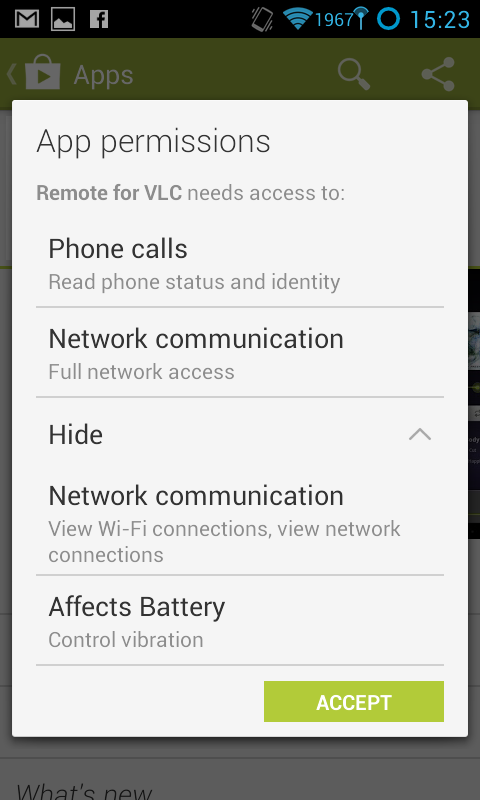
\includegraphics[scale=0.4, bb=0 0 480
800]{img/vlc_permissions_install.png}
\caption{Install time permissions for \emph{Remote for VLC} as listed by
\texttt{AndroidManifest.xml}.}
\label{fig:install-time}
\end{figure}
\\
\noindent This leads to a question concerning the trust of the manifest - so
far the onus is placed on the developer to report the permissions that the application needs to run. What if a developer
were to \textbf{not} list a certain permission (such as requesting superuser
access?). \textbf{GetRIL} is an application which requires the superuser
permission, however, it seems that the developer forgot to add this to the
manifest. The operating system intercepts the request and displays a very stark
warning as seen in \textbf{Figure \ref{fig:not_declared_in_manifest}}. 
\\
\begin{figure}[htb]
\centering
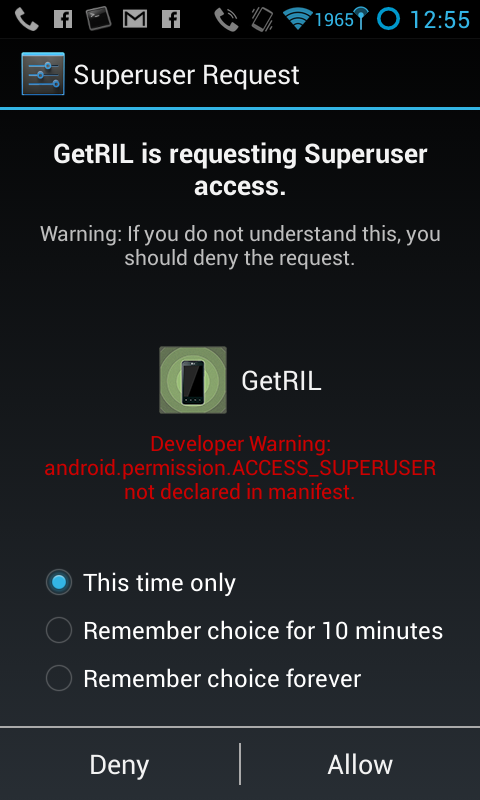
\includegraphics[scale=0.4, bb=0 0 480
800]{img/not_declared_in_manifest.png}
\caption{Superuser permission was not declared in the
\texttt{AndroidManifest.xml} in \emph{GetRIL}.}
\label{fig:not_declared_in_manifest}
\end{figure} 

\noindent Signed certificate files are used to certify whether software is
legitimate or not, and Android disallows unsigned software to be installed by default.
Installing unsigned files requires delving into the system settings, and a
warning message advising the user of unsafe practices appears when disabling the
signature checks. \textbf{Figure \ref{fig:unknown_sources}} shows the checkbox
for enabling the installation from unknown sources. \textbf{Figure
\ref{fig:verisign}} shows one of the VeriSign Certificate Authorities
certificates which are installed by default, as well as a big \emph{disable}
button enabling a user to cease trusting the CA.
\\
\begin{figure}[htb]
\centering
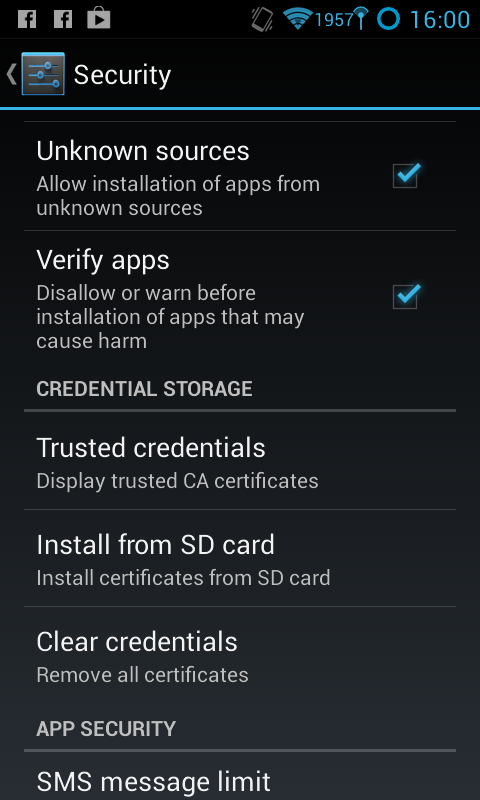
\includegraphics[scale=0.4, bb=0 0 480
800]{img/unknown_sources.png}
\caption{Nested deep in the security settings is the option to allow
installation of applications from \emph{unknown sources}.}
\label{fig:unknown_sources}
\end{figure} 
\begin{figure}[htb]
\centering
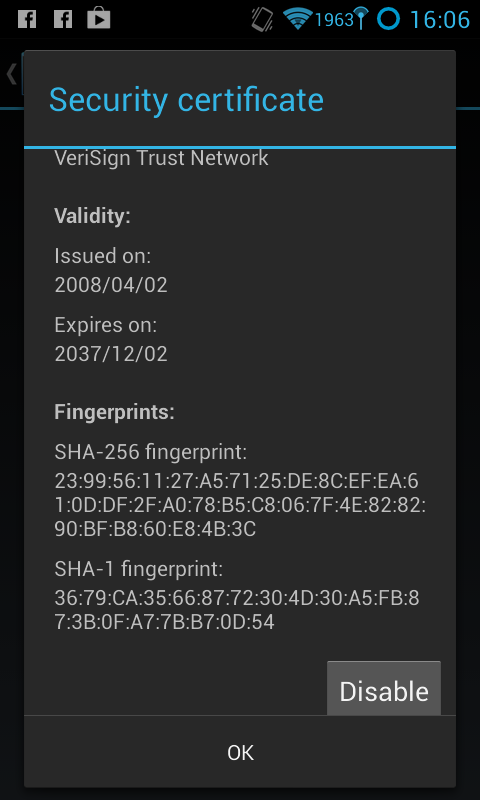
\includegraphics[scale=0.4, bb=0 0 480
800]{img/verisign.png}
\caption{One of VeriSign's CA certificates, and SHA-1 and SHA-256 fingerprints,
along with a button to disable should the user no longer trust this CA.}
\label{fig:verisign}
\end{figure}
\\
\noindent Host key authentication prevents a device being plugged into a PC and
an APK being pushed to the device because unrecognised devices are refused
connection.
\\
\noindent Android 2.2 and up permits \emph{corporate administrators} to lock
down devices such that only specific staff may install software, however this
requires tight integration with the Google Apps ecosystem which the author is
still only just setting up, and without a secondary device with which to
experiment, the author is reluctant to experiment with features that could lock
him out of his own device. Google describes the Device Administration API as
being able
to\footnote{http://developer.android.com/guide/topics/admin/device-admin.html}:
\begin{itemize}
  \item Implement policies
    \begin{itemize}
      \item Password strength
      \item Require storage encryption
      \item Disable Camera
     \end{itemize}
  \item Security applications that do remote wipe
  \item Device management services and applications 
\end{itemize}

\section{Risk Evaluation}
In the default state, the greatest risk comes from the physical security of a
device. The default state of a device is that the device itself has no PIN,
passphrase or pattern to lock / unlock the device, however also are typically
not running any daemons that are likely to be exploitable.
\\
\\
\noindent There are quite reasonable safeguards to prevent a remote attacker
from installing software to exploit a device, and most users are reasonably wary
enough to not physically hand a phone over to someone who is untrusted.

\section{Conclusion}
Social engineering an attack on a user to install malicious software on a device
remains the easiest method of attack. Even so, the permissions at install time
will alert the user as to what the software has the capability of doing. Taking
the earlier example of an application to act as replacement keyboard, a user
\textbf{should} ask \emph{``Why does a keyboard need Internet access? Why does it
need to send an SMS?''}. Other applications, such as launchers which download
news and social media, as well as having dialers to make dialing a phone call
(say you're driving a car) easier make asking these questions somewhat harder.
\\
\\
\noindent Anecdotal evidence suggests that most users do not actually read these
permissions and usually confirm installation.
\\
\\
\noindent For a brand new device, simply exercising caution and putting a
passphrase or PIN to unlock the device should suffice for most users.

\end{document}